\section{TeraHeap for Parallel Scavenge GC}
\label{teraheap:sec:impl}

We implement \teraheapName{} in OpenJDK8 (jdk8u345) and OpenJDK17 (jdk17u067), both
long-term support versions, by extending the Parallel Scavenge
(PS)~\cite{jones:gc_handbook} garbage collector and exporting \teraheapName{}'s interface
through the \emph{Unsafe} class to frameworks.
%
We select PS over the Garbage-First garbage collector (G1GC)~\cite{zhao:g1}
because PS does not result in out-of-memory (OOM) errors when running with small
heap sizes relative to datasets that contain large-sized (humongous) objects.
Our evaluation (Figure~\ref{fig:g1}) shows that G1GC is prone to OOM errors due
to region fragmentation caused by humongous objects.

\paragraph{\textbf{Post-write barriers}}
PS uses a post-write barrier and a card table to track updates in old
generation objects that generate references to young objects. Such
updates may originate from interpreted or JIT compiled methods with
the C1 and C2 JVM compilers. When a mutator thread updates an object
in the old generation, it also performs post-write barrier that
updates the corresponding entry in the H1 card table.

To examine if the mutator thread updates an object that belongs to H1
or H2, we use an additional range check for references in the
post-write barrier. This reference range check selects the appropriate
(H1 or H2) card table, which we then mark with the existing post-write
barrier code. We extend post-write barriers by augmenting the
template-based interpreter and the JIT compilers to generate assembly
code for the necessary checks. We evaluate the overhead of our
modifications to post-write barriers using the DaCapo benchmark
suite~\cite{blackburn:dacapo}. The overhead is small and within 3\% of
total execution time on average across all benchmarks. The additional
overhead is zero for applications that do not enable
\texttt{EnableTeraHeap}.

\paragraph{\textbf{Minor \teraheapGC}}
In minor \teraheapGC, we perform two key tasks during liveness analysis.
Firstly, we introduce a reference range check in the liveness analysis
to fence PS from scanning objects in H2. Secondly, we prevent the
reclamation of H1 objects referred from H2 objects (backward
references) by scanning the H2 card table. Also, we update the
backward references and H2 card values.

\paragraph{\textbf{Major \teraheapGC in Java8}}
The single-threaded version of major \teraheapGC in PS, also known as Serial
old, consists of four main phases, which we extend to support \teraheapName{}.
In the first phase (marking), PS recursively scans both generations
starting from roots (e.g., thread stacks) and marks live objects. PS
assigns a new memory location to each live object in the second phase
of major \teraheapGC (pre-compaction). In the third phase
(pointer-adjustment), PS adjusts the references of each object to
point to the new location of the objects as determined in
pre-compaction phase. In the final phase (compaction), PS moves
objects to their new locations.

We extend the marking phase to perform five extra tasks. At the beginning of the
marking phase, we reset all the \texttt{live} bits of the H2 regions. We mark
all objects in H1 that are referenced by H2 as live. We add a reference range
check (similar to minor \teraheapGC) that detects forward references (H1 to H2) to fence
PS from scanning objects in H2, and we set the \texttt{live} bit of the
corresponding region. We identify the root objects tagged with a label through
\teraheapName{} interface and calculate their transitive closure. Finally, we free all
dead regions in H2.

To determine which objects found in the marking phase should be moved
to H2, we extend the pre-compaction phase. We assign these objects an
address from H2 using their label.

We prolong the pointer adjustment phase to perform three additional
operations:
%
(1) we adjust all backward references to the new object locations in
H1,
%
(2) we identify the newly cross-region references, and
%
(3) we track the newly created backward references.
%
For this purpose, when we adjust the references of H1 objects that are
candidates for H2 transfer, we check if they reference an existing H2
region or point to an H1 object. If a candidate object references an
existing H2 region, we update the dependency list of the H2 region in
which the candidate object is transferred. Also, in case the candidate
object has a reference to an H1 object, we mark the appropriate entry
in the H2 card table as dirty.

Finally, in the compaction phase, PS moves objects to H2.

\paragraph{\textbf{Major \teraheapGC in Java17}}
The major \teraheapGC in PS in OpenJKD17 consists of three main phases, which
we extend to support \teraheapName{}. In the first phase (marking), parallel
\teraheapGC threads scan both generations starting from roots (e.g., stacks
from mutator threads, global variables, JIT methods) and mark live
objects. In the second phase (summary), PS divides the heap into
\SI{512}{KB} regions and calculates sequentially for each region a
destination address. In the third phase (compaction), firstly, the \teraheapGC
threads adjust in parallel the roots to point to the new location of
the objects as determined in the summary phase. Next, the \teraheapGC threads
process the regions in parallel and copy the live objects to the
beginning of each space (old generation and from-space in young
generation).

\begin{figure}
  \subfloat[Marking Phase]{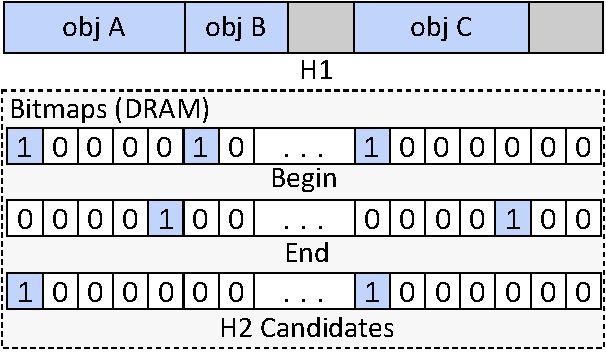
\includegraphics[width=0.42\linewidth]{teraheap/fig/marking.pdf}}
  \hspace{15pt}
  \subfloat[Precompact Phase]{
    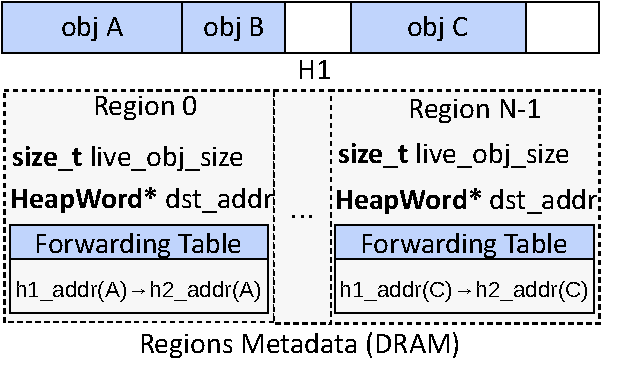
\includegraphics[width=0.4\linewidth]{teraheap/fig/h2_precompact.pdf}
  }
	\caption{Extensions in PS garbage collector to work with \teraheapName{}}´
	\label{fig:jdk17}
\end{figure}

PS uses two marking bitmaps to map the entire heap during the marking phase, as
shown in Figure~\ref{fig:jdk17}(a). Each bit in the bitmap corresponds to
\SI{64}{bits} of the heap because of the \SI{8}{byte} alignment of fields in a
JVM object. The first bitmap marks the start address of each live object, and
the second bitmap marks the end address. To calculate the object's size, we
multiply the bits between the enabled bits in the start and end bitmaps by
eight. The collector divides the heap space into regions of \SI{512}{KB} and
maintains metadata for each object in DRAM. It updates the metadata of the
region the object belongs to when it marks an object as live.

In our implementation, we extend PS to maintain a third bitmap during
the marking phase, as shown in Figure~\ref{fig:jdk17}(a). This bitmap
tracks the start address of the objects that should be moved to the
second heap (H2 candidates). In addition to the five extra tasks
described in the major \teraheapGC of Java8, we update the third bitmap for
each object in the transitive closure. The third bitmap is essential
in the H2 migration process and for updating H1 objects that reference
H2 candidate objects, as it enables us to identify H2 candidate
objects efficiently.

To make the space of H2 candidate objects available to the garbage collector to
compact live H1 objects, we extend the metadata of each region to maintain a
forwarding table for H2 candidate objects.  In the case of an H1 object
referencing an H2 candidate object, when we adjust its references, we perform a
lookup in the forwarding table to find the new address of the candidate object
in H2. Each entry of the forwarding tables, as shown in
Figure~\ref{fig:jdk17}(b) is \SI{16}{bytes} because it stores for each
candidate the old address in H1 (\SI{8}{bytes}) and their new address in H2
(\SI{8}{bytes}). We use our own allocator to optimize the memory allocation for
the forwarding table. This approach avoids the overhead of multiple calls to
the system \texttt{malloc()} and \texttt{free()} functions and can
significantly improve performance. We note that forwarding tables might
increase the metadata of JVM when we have hundreds of millions of objects to
transfer to H2 in one \teraheapGC cycle.  Thus, we limit the size of the forwarding
tables to \SI{1}{GB} by transferring to H2 up to 67,108,864 objects per major
\teraheapGC cycle.

Avoiding forwarding tables requires storing inside the header of H2
candidate objects their new address in H2 (forwarding information).
Although this approach avoids using extra DRAM space for metadata, it
delays the time when the space of H2 candidates can be reclaimed. The
\teraheapGC must first process all objects that may reference the H2 candidate
objects and then reclaim their space. For this purpose we need to
split the compaction phase of PS into two sub-phases: a phase to adjust
the references of the objects and a phase to compact H1 objects. We
leave this investigation for future work.

At the start of the summary phase, we determine which objects found in
the marking phase should be moved to H2. We scan the bitmap for H2
candidates, and for each candidate, we get an address from the H2
allocator. We assign this address to the forwarding table of the
region.  Next, we remove the candidate objects from the marking
bitmaps (start and end) and decrease the total size of the live
objects in the corresponding region.

Before we compact H1 objects, we add one extra phase that adjusts the
backward references and moves candidate objects to H2. In addition to
the movement of the objects in H2, in this phase, we perform the same
operations as described in the pointer adjustment phase of the major
\teraheapGC in Java8. Next, the PS continues to compact and adjust H1
candidate objects. At the end of the major \teraheapGC, we reclaim all the
allocated memory for the forwarding tables and clear marking bitmaps.

\subsection{Applicability to Other Garbage Collectors}
% \teraheapName{} can also be ported to other garbage collectors, such as G1GC. It is
% implemented as a new instance class inside the OpenJDK, providing an API that
% each garbage collector can use. For example, they check if an object belongs to
% H2 or mark an H2 region as active because it contains live objects. These API
% function calls need to be inserted into the source code of each garbage
% collector, where each collector performs liveness analysis, assigns new
% addresses to objects, makes object pointer adjustments, and moves objects to
% their new location. JVM developers also need to extend the post-write barrier of
% each garbage collector in the interpreter and JIT compilers to update the H2
% card table. As part of future work, we plan to port \teraheapName{} to G1GC and assess
% its performance in latency-sensitive frameworks, such as
% Cassandra~\cite{teraheap:cassandra} and Lucene~\cite{lucene}.
\teraheapName{} can be ported to work with other garbage collectors, such as G1GC. It is
implemented as a new class within OpenJDK, providing an API for garbage
collectors. For example, garbage collector developers can use this API to check
whether an object belongs to the H2 or to mark an H2 region as live when it
contains live objects. Developers must insert these API calls into the source
code of each garbage collector, specifically at the points where liveness
analysis is performed, new object addresses are assigned, object pointers are
adjusted, and objects are moved to new locations. Furthermore, JVM developers
need to modify the post-write barriers in both the interpreter and JIT compilers
to update the H2 card table. In future work, we plan to port \teraheapName{} to G1GC and
evaluate its performance in latency-sensitive applications, such as
Cassandra~\cite{teraheap:cassandra} and Lucene~\cite{lucene}.
